\section{Struktur der einzelnen (Sub-)Elemente}\label{struktur_elemente_style}

In diesem Abschnitt geht es um die Standardisierung des einzelnen Elemente
und Subelemente hinsichtlich ihres Aufbaus und ihrer grunds"atzlichen
Konzeption.

\vspace{3mm}

\subsection{Philosophie}

"Ubergeordnete Metas f"ur diese Festlegungen sind:

\begin{list_sabina}
\item
\textbf{listenartig}
\item
\textbf{bildhaft}
\item
\textbf{objektorientiert}
\item
\textbf{"ubersichtlich}
\item
\textbf{modular}
\item
\textbf{standalone}
\end{list_sabina}


\subsection{Allgemeine Vorbemerkungen}

\begin{list_sabina}
\item
Bei den i.f. dargestellten Skizzen handelt es sich um \textbf{funktionale
Beschreibungen} und Kapselungsanweisungen des Sachverhaltes, 
nicht um fertige Layoutanweisungen. 
\item
Die Skizzen zu den einzelnen Elementen sind u.U. noch nicht vollst"andig,
d.h., es existieren m"oglicherweise Theoreme etc., die mit keiner
der angebotenen Umgebungen abbildbar sind, weil sie einen v"ollig anderen
inneren Aufbau haben.\\
Treten solche F"alle auf, werden ggf. entsprechende Umgebungen nachentwickelt.
\item
Innerhalb der einzelnen ``Bl"ocke'' der folgenden Umgebungen f"ur die einzelnen
(Sub-)Elemente (z.B. ``Forderungen'' beim Theorem, 
s. S. \pageref{block_theorem_impl_single_h_v} ff.) sollte stets so ``listenartig'' wie m"oglich 
geschrieben werden.
\end{list_sabina}


\subsection{Alle Elemente auf einem Blick}

\textbf{Zur Orientierung die vorhandenen Elemente in der
"Ubersicht\footnote{Die Idee einer ``Zusammenfassung'' (z.B. von
Eigenschaften etc.) wurde hier noch nicht aufgenommen, ist aber nicht
vergessen! Es erscheint derzeit sinnvoller, zun"achst einige Module
bis auf die Elementebene hinunter zu analysieren, um daraus das
Auftreten dieser ``Zusammenfassungen'' und die innere Struktur besser
absch"atzen zu k"onnen: z.B. ist derzeit unklar, ob solche
``Zusammenfassungen'' immer existieren oder nur manchmal, ob sie auf
Modulebene leben oder aber auch auf kleineren und/oder gr"o"seren
Hierarchie-Einheiten usw.}:}\label{zusammenfassungselemente_footnote}

\begin{enumerate}
    \item Motivation \hspace{32.7mm} (M) \\[-4ex]
    \item Definition \hspace{34.4mm} (D) \\[-5ex]
    \item Theorem \hspace{35.9mm} (T) \\[-5ex]
    \item Lemma (Hilfssatz) \hspace{19.9mm} (L) \\[-5ex]
    \item Algorithmus \hspace{30.2mm} (Al) \\[-4ex]
    \item Anwendung (naturw.) \hspace{14mm} (A)
\end{enumerate}

\clearpage

Die o.g. Elemente zerfallen in die oben angedeuteten drei Gruppen:

\begin{list_sabina}

        \item Motivation:
        \begin{sub_list_sabina}
                \item 
                mathematisch nicht hart
                \item 
                nat"urlicher Anfang einer Thematik
        \end{sub_list_sabina}

        \item Definition, Theorem, Lemma, Algorithmus: 
        \begin{sub_list_sabina}
                \item 
                mathematisch hart
                \item 
                Kernteil einer Thematik
                \item 
                logisch aufeinander aufbauend, voneinander abh"angend
        \end{sub_list_sabina}

        \item Anwendung:
        \begin{sub_list_sabina}
                \item 
                mathematisch sachlich
                \item 
                nat"urlicher Schlu"s einer Thematik
        \end{sub_list_sabina}

\end{list_sabina}

Diese Gruppen zeichnen sich i.f. auch in ihrer Struktur deutlich ab.


\subsubsection{Alle Subelemente auf einem Blick}

\textbf{Zur Orientierung die vorhandenen Subelemente in der "Ubersicht:}

\begin{enumerate}
    \item Herleitung\\[-4ex]
    \item Beweis\\[-4ex]
    \item Historisches\\[-5ex]
    \item Bemerkung\\[-5ex]
    \item Motivation (zum Hauptelement)\\[-4ex]
    \item Visualisierung\\[-5ex]
    \item Beispiel\\[-5ex]
    \item Tabelle\footnotemark
\end{enumerate}\footnotetext{Tabelle: im Sinn einer (Bsp.)Liste, einer Wertetabelle, ...}

Die o.g. Elemente zerfallen in die oben angedeuteten vier Gruppen:

\begin{list_sabina}

        \item Herleitung:
        \begin{sub_list_sabina}
                \item 
                mathematisch hart
                \item 
                geht einem Theorem/Lemma voran
        \end{sub_list_sabina}

        \item Beweis:
        \begin{sub_list_sabina}
                \item 
                mathematisch hart
                \item 
                folgt einem Theorem/Lemma
        \end{sub_list_sabina}

        \item Historisches, Bemerkung, Motivation (zum Hauptelement): 
        \begin{sub_list_sabina}
                \item 
                mathematisch nicht hart, eher leicht ``geschw"atzig''
        \end{sub_list_sabina}

        \item Visualisierung, Beispiel, Tabelle:
        \begin{sub_list_sabina}
                \item 
                mathematisch sachlich
        \end{sub_list_sabina}

\end{list_sabina}

Auch diese Gruppen zeichnen sich i.f. in ihrer Struktur deutlich ab.


\clearpage

\subsection{Die Elemente im einzelnen}

\subsubsection{Definition}

In einer Definition wird i.a. nur \textbf{ein} zu definierender Begriff 
eingef"uhrt (voll-modular).
Ausnahmen sind lediglich dann zul"assig, wenn die betreffenden 
Definitionen praktisch ``immer'' gemeinsam eingef"uhrt werden und 
dadurch kein wirklicher Widerspruch zur Modularit"at entsteht, wie etwa bei
``Zeilenrang und Spaltenrang'' (s.u. im Bild: ``Doppeldefinitionen'').
Innerhalb solcher Definitionen werden die einzelnen Teile dann 
numeriert.\\
Verschiedene "aquivalente Definitionen d"urfen \textbf{niemals} 
in einer einzigen Definition dargestellt werden\footnote{Sie m"ussen
in getrennten Definitionen vorgestellt werden, zus"atzlich mu"s ein
Satz formuliert werden, der die "Aquivalenz der beiden Aussagen beweist.}
(f"ur ``"Ubersichtsdarstellungen'' etwa verschiedener "aquivalenter
Definitionen werden zus"atzliche Zusammenhangselemente (vergleiche
Fu"snote S. \pageref{zusammenfassungselemente_footnote})
entwickelt).

\vspace{5mm}

Die bildhaften/strukturierten Aufbauten folgen den u.s. Schemata:

\vspace{5mm}

\textbf{Der Normalfall:}

\begin{center}
\ifx\pdfoutput\undefined
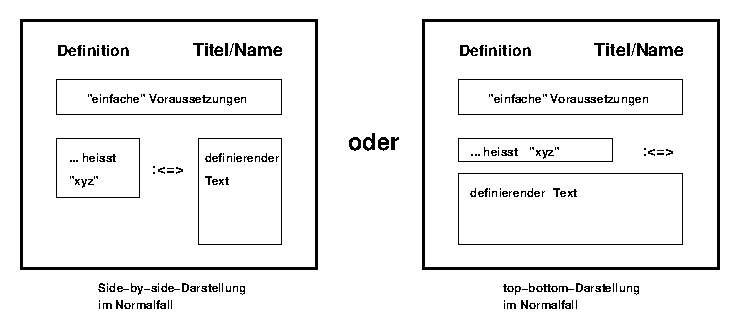
\epsfig{file=Skizzen/block_def_single_h_v.eps} 
\else
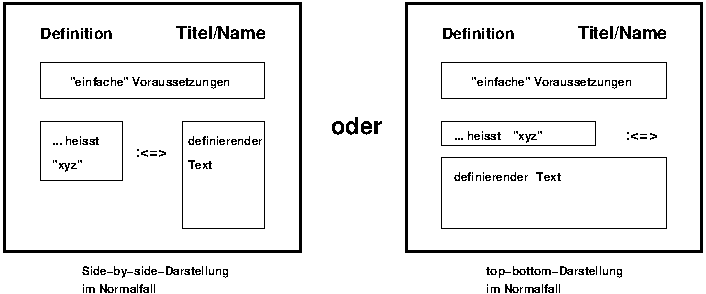
\includegraphics{Skizzen/block_def_single_h_v.pdf}
\fi
\end{center}

\textbf{Ausnahmefall Doppeldefinitionen:}

\begin{center}
\ifx\pdfoutput\undefined
   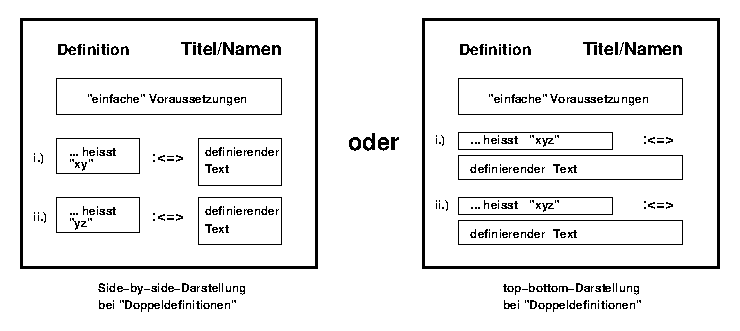
\epsfig{file=Skizzen/block_def_multi_h_v.eps} 
\else
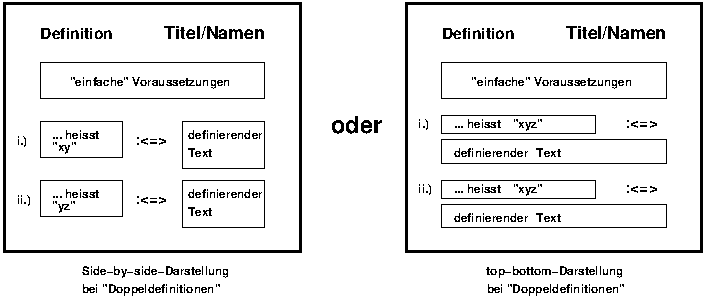
\includegraphics{Skizzen/block_def_multi_h_v.pdf} 
\fi
\end{center}

\textbf{Ausnahmefall Tripeldefinitionen} usw.: folgt entsprechend.

\vspace{5mm}

Definitionen tragen \textbf{grunds"atzlich} einen Titel; dieser
besteht i.a. aus dem Namen des zu definierenden Gegenstandes.

\clearpage

F"ur Definitionen, die sich in obiges Schema nicht einordnen lassen
(ca. 3\% !!!) steht eine Freestyle-Umgebung zur Verf"ugung, die aber
nur diese absoluten Ausnahmef"alle regelt:

\textbf{Freestyle - einfache Definition:}

\begin{center}
\ifx\pdfoutput\undefined
   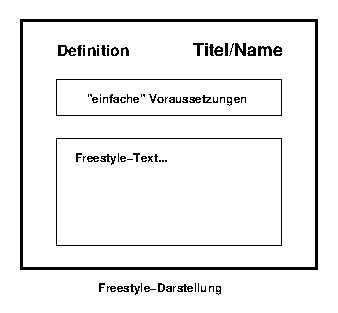
\epsfig{file=Skizzen/block_def_single_free.eps} 
\else
   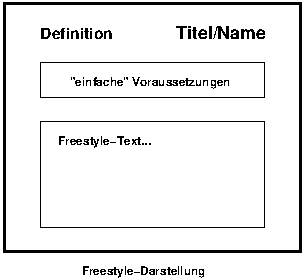
\includegraphics{Skizzen/block_def_single_free.pdf} 
\fi
\end{center}

\textbf{Freestyle - Ausnahmefall Doppeldefinitionen:}

\begin{center}
\ifx\pdfoutput\undefined
   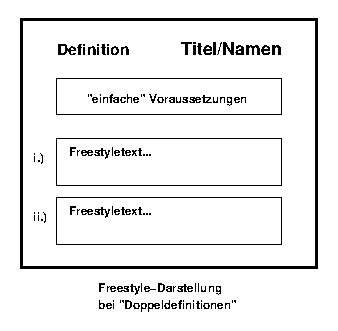
\epsfig{file=Skizzen/block_def_multi_free.eps} 
\else
   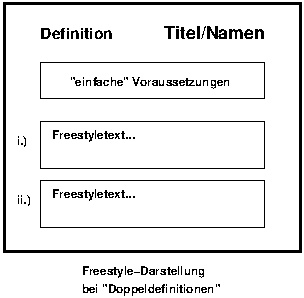
\includegraphics{Skizzen/block_def_multi_free.pdf} 
\fi
\end{center}

\textbf{Freestyle - Ausnahmefall Tripeldefinitionen} usw.: folgt entsprechend.


\clearpage



\subsubsection{Theoreme}\label{style_theoreme}

In einem Theorem wird i.a. genau \textbf{eine} Aussage vorgestellt.\\
Ausnahmen sind jedoch dann zul"assig, wenn die betreffenden Aussagen
inhaltlich so stark verkn"uft sind, da"s sie praktisch ``immer''
gemeinsam zitiert werden.

\vspace{5mm}

Die bildhaften/strukturierten Aufbauten folgen den u.s. Schemata:

\vspace{5mm}

\textbf{Der Normalfall; Implikationen und S"atze f"ur Eigenschaften:}

\begin{center}\label{block_theorem_impl_single_h_v}
\ifx\pdfoutput\undefined
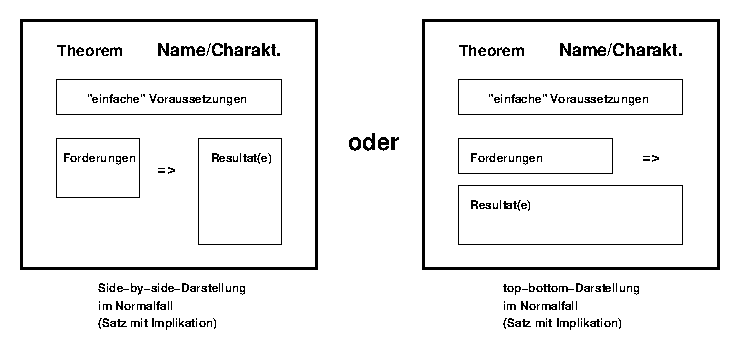
\epsfig{file=Skizzen/block_theorem_impl_single_h_v.eps} 
\else
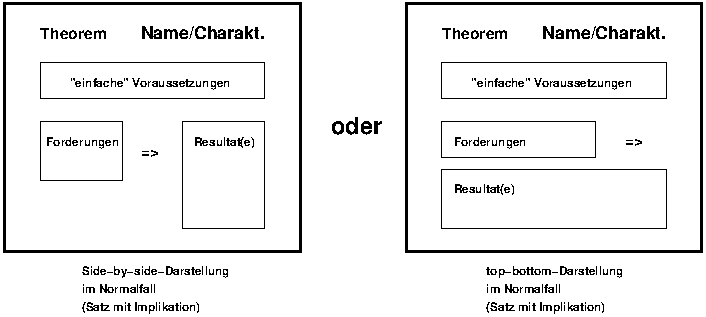
\includegraphics{Skizzen/block_theorem_impl_single_h_v.pdf} 
\fi
\end{center}

\begin{center}
\ifx\pdfoutput\undefined
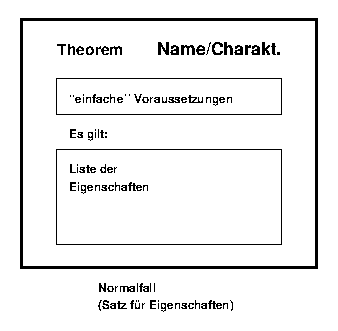
\epsfig{file=Skizzen/block_theorem_eigen_single_h_v.eps} 
\else
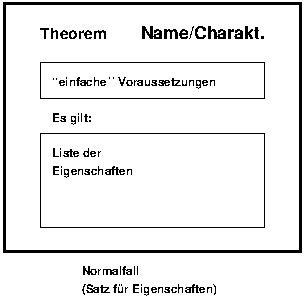
\includegraphics{Skizzen/block_theorem_eigen_single_h_v.pdf} 
\fi
\end{center}


\clearpage

\textbf{Der Normalfall; "Aquivalenzen und S"atze f"ur "aquivalente Eigenschaften:}

\begin{center}
\ifx\pdfoutput\undefined
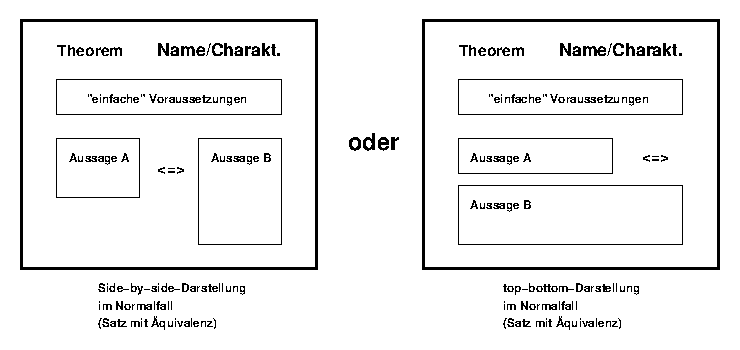
\epsfig{file=Skizzen/block_theorem_aequi_single_h_v.eps} 
\else
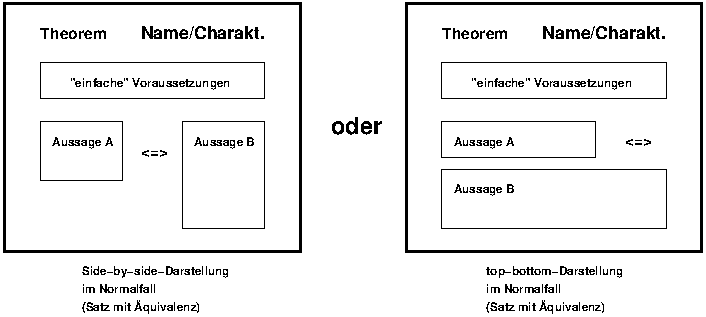
\includegraphics{Skizzen/block_theorem_aequi_single_h_v.pdf} 
\fi
\end{center}

\begin{center}
\ifx\pdfoutput\undefined
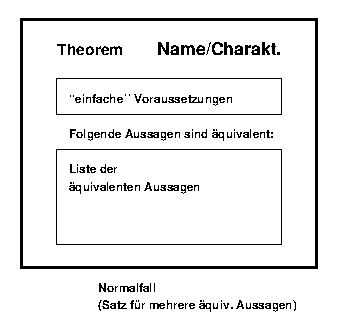
\epsfig{file=Skizzen/block_theorem_multaequi_h_v.eps} 
\else
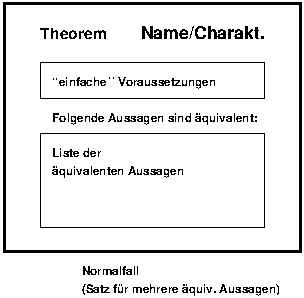
\includegraphics{Skizzen/block_theorem_multaequi_h_v.pdf} 
\fi
\end{center}

\clearpage


\textbf{Ausnahmefall Doppeltheorem; Implikationen:}

\begin{center}
\ifx\pdfoutput\undefined
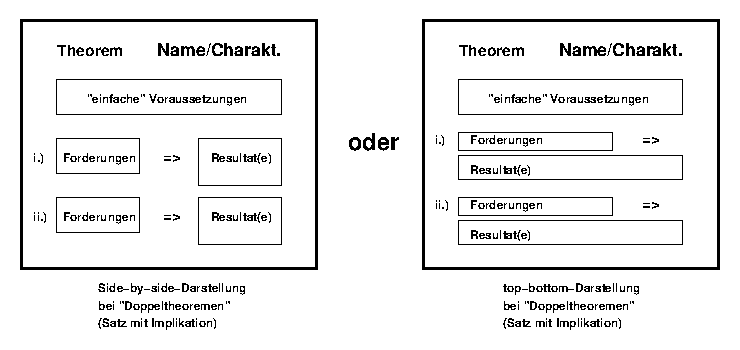
\epsfig{file=Skizzen/block_theorem_impl_multi_h_v.eps} 
\else
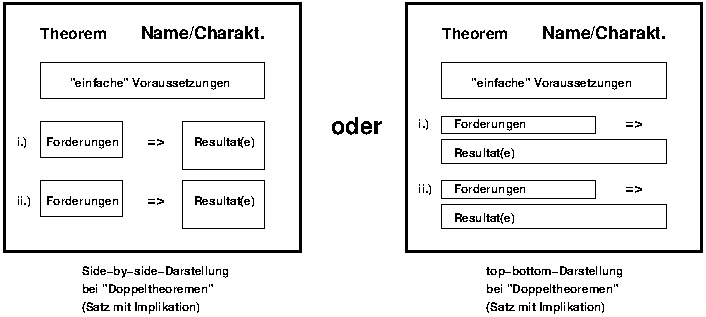
\includegraphics{Skizzen/block_theorem_impl_multi_h_v.pdf} 
\fi
\end{center}

\textbf{Ausnahmefall Doppeltheorem; "Aquivalenzen:}

\begin{center}
\ifx\pdfoutput\undefined
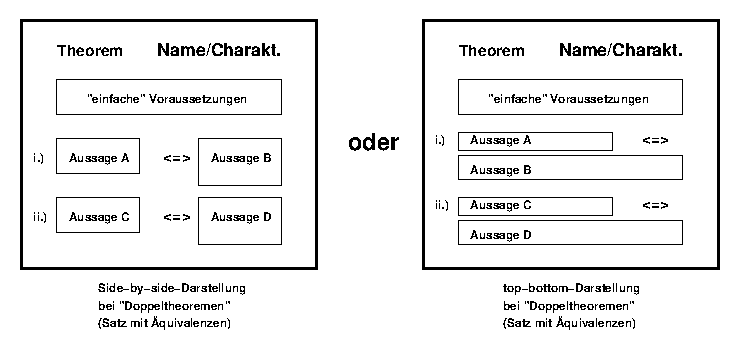
\epsfig{file=Skizzen/block_theorem_aequi_multi_h_v.eps} 
 \else
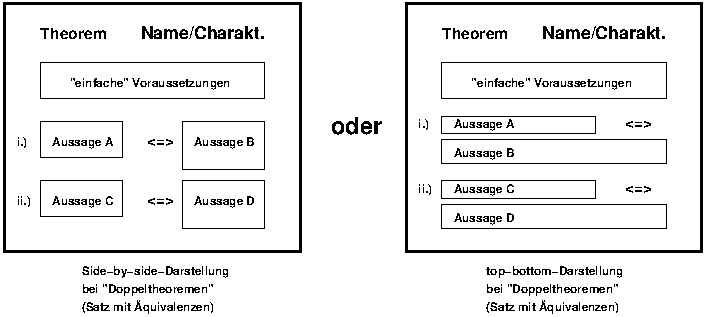
\includegraphics{Skizzen/block_theorem_aequi_multi_h_v.pdf} 
\fi
\end{center}


\textbf{Ausnahmefall Tripeltheorem} usw.: folgt entsprechend.

\vspace{5mm}

Theoreme tragen \textbf{optional} einen Titel; dieser besteht
i.a. entweder aus dem ``offiziellen Namen'' eines Satzes (etwa ``Satz
von Bolzano-Weierstra"s'') oder aus einer inhaltlichen Charakterisierung
(etwa ``Grundlegende Eigenschaften der e-Funktion'')\footnote{Es ist
offensichtlich, da"s es nicht f"ur jeden Satz pr"agnante Titel in
obigem Sinne gibt: da solche Titel aber zur Orientierung sehr
hilfreich sind, sollte diese Angabe soweit m"oglich stets erfolgen.}.

\clearpage


\subsubsection{Lemmata}

F"ur Lemmata (zu verstehen als Hilfssatz) gilt inhaltlich exakt
dasselbe wie f"ur Theoreme; es werden dieselben environments
ben"otigt, es gelten dieselben Regeln zur Namensvergabe etc.

\vspace{5mm}

Somit folgen auch die bildhaften Aufbauten den bei ``Theorem''
(s. Kap. \ref{style_theoreme}) skizzierten Schemata.%\\
%Einzige Ausnahmen: die Umgebungen ``Satz f"ur Eigenschaften'' sowie ``Satz
%f"ur mehrere "aquivalente Aussagen�� werden f"ur Lemmata nicht vorgehalten
%(``Eigenschaften'' haben keinen Hilfssatzcharakter, mehrere "aquivalente
%Aussagen sind i.a. so wichtig, da"s sie Theorem-Charakter (nicht
%Hilfssatzcharakter) haben).

\clearpage


\subsubsection{Algorithmen}

In einem Algorithmus wird genau \textbf{ein} Algorithmus/\textbf{ein} 
Rechenverfahren vorgestellt.\\
Ausnahmen sind nicht vorgesehen, zum einen aus Gr"unden einer m"oglichst
weitreichenden Modularisierung, zum anderen, weil i.a. schon ein einzelner
Algorithmus ``komplex'' und damit ``seitenf"ullend'' ist.

Die bildhaften/strukturierten Aufbauten folgen den u.s. Schemata:

\vspace{5mm}

\textbf{Algorithmus:}

\begin{center}
\ifx\pdfoutput\undefined
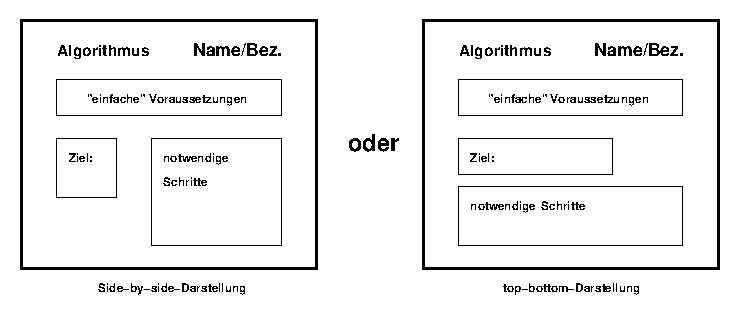
\epsfig{file=Skizzen/block_algo_single_h_v.eps} 
\else
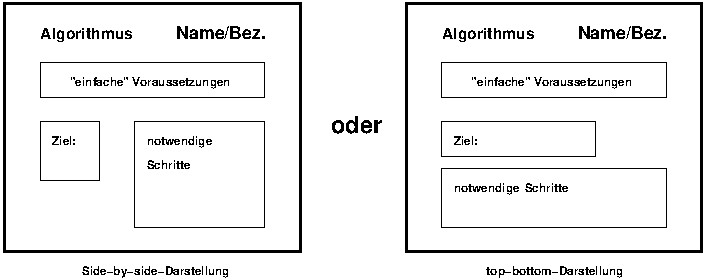
\includegraphics{Skizzen/block_algo_single_h_v.pdf} 
\fi
\end{center}


\clearpage

\subsubsection{Motivation}

\begin{list_sabina}\label{sw_motivation}
\item
\textit{kein fester} bildhafter Aufbau
\item
Ans"atze f"ur wiederkehrende Ideen bei der Gestaltung:
        \begin{sub_list_sabina}
        \item
        ``Duell'' oder Unterhaltung zweier Figuren (``Mumie'' und ihr Counterpart) 
        \item
        ...
        \end{sub_list_sabina}
\end{list_sabina}


\subsubsection{Anwendungen}

\begin{list_sabina}
\item
\textit{kein fester} bildhafter Aufbau, aber bildhafter Aufbau dennoch
angestrebt\footnote{Zum gegenw"artigen Zeitpunkt erscheint es noch zu
fr"uh, hier geeignete Umgebungen zu definieren: zun"achst m"ussten
exemplarisch einige Anwendungen auf innere Strukturen untersucht
werden.}
\end{list_sabina}


\clearpage

\subsection{Die Subelemente im einzelnen}

\subsubsection{Herleitung und Beweis}\label{block_herl_bew_struct}

Herleitungen/Beweise werden grunds"atzlich\footnote{Diese Skizze
mu"s immer erfolgen, um f"ur den Lernenden
zun"achst den Focus auf die ``zentrale Idee'', 
den ``wichtigen Beweisinput'', zu setzen.} 
zun"achst mit ihren wesentlichen Ideen skizziert;
die Skizze erfolgt listenartig.\\
Beim "Uberfahren des entsprechenden Listeneintrages k"onnen 
die zugeh"origen Details z.B. ``seitlich 
herausgefahren'' werden\footnote{Eine komplette Version, alle
Beweisteile untereinander, wird zus"atzlich angeboten.}.

Die bildhaften/strukturierten Aufbauten folgen den u.s. Schemata:

\begin{center}
\ifx\pdfoutput\undefined
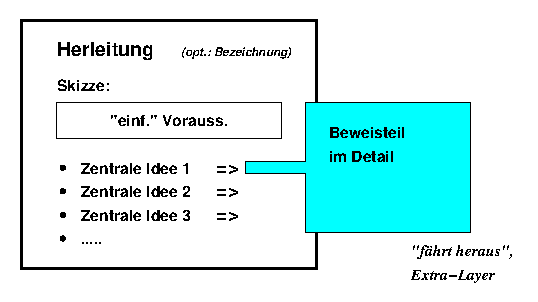
\epsfig{file=Skizzen/block_herl_struct.eps} 
\else
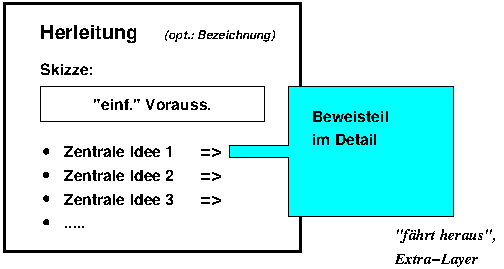
\includegraphics{Skizzen/block_herl_struct.pdf} 
\fi
\end{center}

\begin{center}\label{block_bew_struct}
\ifx\pdfoutput\undefined
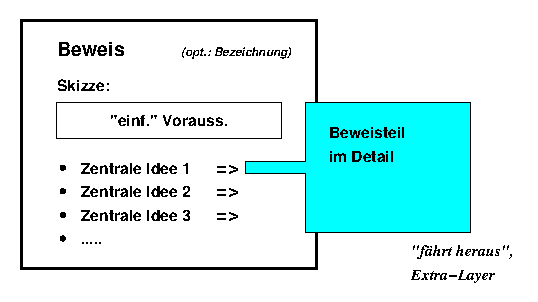
\epsfig{file=Skizzen/block_bew_struct.eps} 
\else
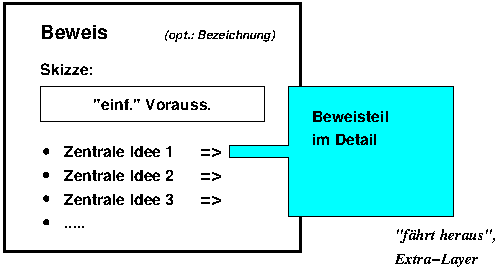
\includegraphics{Skizzen/block_bew_struct.pdf} 
\fi
\end{center}

(Die ``optionale Bezeichnung'' kann verwendet werden, wenn ein
Beweisverfahren unter einem bestimmten Namen bekannt ist oder einen
typischen mathematischen Aspekt tr"agt.)

\clearpage

\subsubsection{Historisches, Bemerkung, Motivation (zum Hauptelement)}

\textbf{Historisches} sollte wie ein wissenschaftlich-historischer
Kurzartikel verfa"st werden\footnote{Wir sind nat"urlich keine
Wissenschaftshistoriker, dennoch sollten unsere ``historischen''
Subelemente nicht so wirken, als h"atte man sie einfach aus ``Mein
kleines Geschichtslexikon'' abgeschrieben.}, ggf. angereichert durch
interaktive, multimediale und spielerische Elemente.

Das Subelement ``Historisches'' mu"s grunds"atzlich so konzeptioniert
werden, da"s es auch f"ur einen Lexikoneintrag (entweder ``alleine''
oder zusammen mit anderen Elementen/Subelementen) verwendet werden
kann.

Aktuell sind folgende ``Auspr"agungen'' dieses Subelementes vorgesehen
(hier dargestellt zusammen mit dem dazugeh"origen Teilen, aus denen das
Subelement dann bestehen soll):

\begin{enumerate}
\item
\textbf{Personen\footnote{Auch ``Gruppen mit Namen'', etwa Bourbaki, 
sind in diesen Sinne ``Personen''...} -- Biographien:}
        \begin{sub_list_sabina}
        \item
        \textbf{Abri"s:} Lebensdaten etc., allg. Daten, zentrales Wirkungsfeld, 
        Zugeh"origkeit zu (mathematischer) Schule (incl. der Lehrer), 
        Einbettung in wissenschaftliches Umfeld
        \item
        \textbf{Math./Fachl. Werk:} "Ubersicht "uber mathematisches/fachliches Gesamtwerk
        mit klar voneinander abgegrenzten einzelnen Abs"atzen;\\
        erg"anzend gibt es jeweils eine detaillierte Darstellung dieser 
        Einzelpunkte\footnotemark.
        \item
        \textbf{"Uberfachl. Bedeutung} (opt.): kulturhistorische Bedeutung, 
        gesamtgesellschaftliches Wirken, Beeinflussung des Lebensweges
        durch politische/gesellschaftliche Gegebenheiten etc.        
	         \item
	         \textbf{Bild}
	         \item
	         \textbf{Lebensdaten}: Zusammenfassung Lebensdaten
        \end{sub_list_sabina}   
\item
\textbf{Mathematische Gebiete, Zweige -- "Ubersichtsdarstellung:}
        \begin{sub_list_sabina}
        \item
        \textbf{Abri"s:} allgemeine Informationen, Daten zur Entwicklung, 
        erstes Auftreten, urspr"ungliche Fragestellung, wichtigste Namen, etc.
        \item
        \addtocounter{footnote}{-1}
        \textbf{Math. Gebiet:} "Ubersicht "uber das mathematische Gebiet
        mit klar voneinander abgegrenzten einzelnen Abs"atzen;\\
        erg"anzend gibt es jeweils eine detaillierte Darstellung dieser 
        Einzelpunkte\footnotemark.
        \item
        \textbf{"Uberfachl. Bedeutung} (opt.): historische Bedeutung, 
        gesamtgesellschaftliche Bedeutung etc.  
        \end{sub_list_sabina}\footnotetext{Die Idee folgt etwa der Darstellung von 
        ``Beweis'' oder ``Herleitung'', allerdings ist die "Ubersicht nicht
        stichwortartig, sondern in ganzen S"atzen formuliert.}   
\item
\textbf{Einzelne bedeutende Resultate\footnote{Hierzu geh"ort etwa eine historische 
Bemerkung zur Bedeutung des Fundamentalsatzes etc., ggf. mit dem entsprechenden Hinweis auf die
beteiligten Personen...}:}
        \begin{sub_list_sabina}
        \item
        \textbf{Einzelner Abschnitt:} (k"urzerer) Text zur entsprechenden Thematik, 
        erstes Auftreten, urspr"ungliche Fragestellung, 
        weiterf"uhrende Hinweise auf Namen, Gebiete etc., insbesondere zum 
        ``dort Weiterlesen''
        \end{sub_list_sabina}   

\end{enumerate}

\clearpage

Die bildhaften/strukturierten Aufbauten folgen den u.s. Schemata:

\begin{center}
\ifx\pdfoutput\undefined
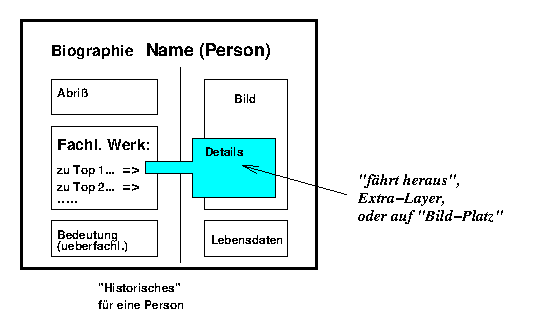
\epsfig{file=Skizzen/block_hist_person_02.eps} 
\else
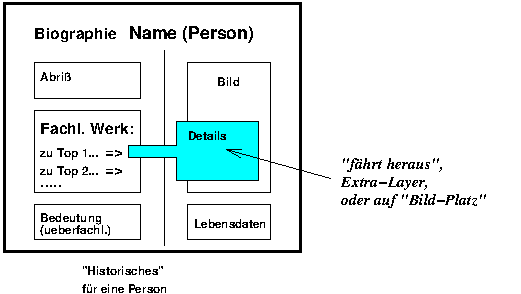
\includegraphics{Skizzen/block_hist_person_02.pdf} 
\fi
\end{center}

\begin{center}
\ifx\pdfoutput\undefined
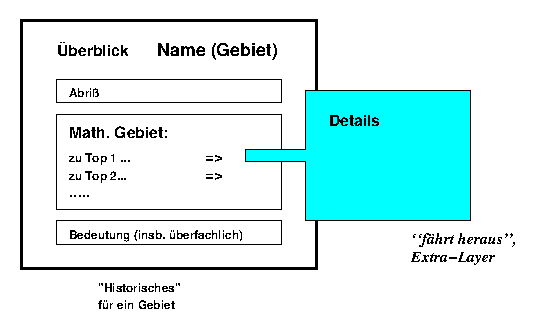
\epsfig{file=Skizzen/block_hist_gebiet.eps} 
\else
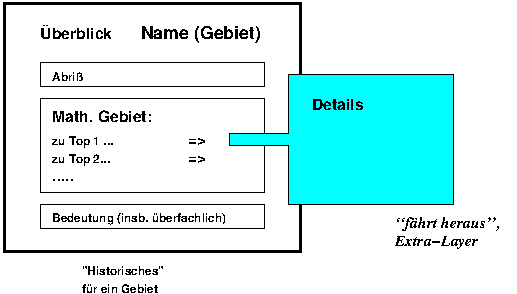
\includegraphics{Skizzen/block_hist_gebiet.pdf} 
\fi
\end{center}

\begin{center}
\ifx\pdfoutput\undefined
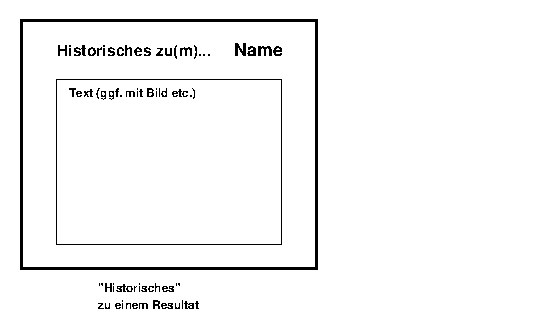
\epsfig{file=Skizzen/block_hist_resultat.eps} 
\else
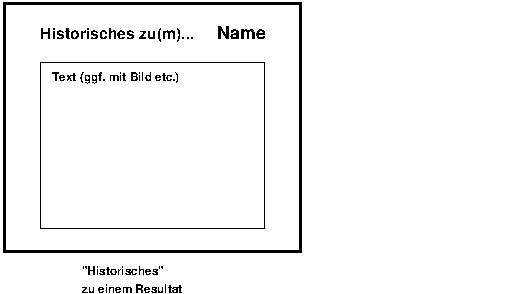
\includegraphics{Skizzen/block_hist_resultat.pdf} 
\fi
\end{center}

\clearpage

\textbf{Bemerkungen} zerfallen inhaltlich in die u.s. Gruppen.\\
Die Gruppenzugeh"origkeit wird "uber zus"atzliche selbstsprechende Icons
angezeigt\footnote{Die Gruppenzugeh"origkeit steht nicht im Vordergrund,
sollte aber einen gewissen Wiedererkennungscharkter haben.}.


\begin{enumerate}
\item
\textbf{Sloppy-Version:}
        \begin{sub_list_sabina}
        \item
        \textbf{Charakter:} ``Sloppy-Version'' des Gegenstandes des Elementes
        \item
        \textbf{Idee/Anspruch:} Kommunizieren der ``grundlegenden Idee'' 
        des Gegenstandes des Elementes 
        \item
        \textbf{Icon:} ...
        \end{sub_list_sabina}   
\item
\textbf{Direkte Bemerkung:}
        \begin{sub_list_sabina}
        \item
        \textbf{Charakter:} Achtung -- Warnung -- Merke
        \item
        \textbf{Idee/Anspruch:} agiert sehr ``direkt'' auf dem Element:
        Hinweis auf typische Fehler und Mi"sverst"andnisse, Merks"atze etc.
        \item
        \textbf{Icon:} gro"ses Ausrufezeichen 
        \end{sub_list_sabina}   
\item
\textbf{Reflektierende Bemerkung:}
        \begin{sub_list_sabina}
        \item
        \textbf{Charakter:} ``Lautes (Nach-)Denken'' "uber den Gegenstand des Elementes
        \item
        \textbf{Idee/Anspruch:} reflektiert den Gegenstand des Elementes, hinterfragt, 
        beleuchtet einzelne Aspekte...  
        \item
        \textbf{Icon:} ...
        \end{sub_list_sabina}   
\item
\textbf{Assoziative Bemerkung:}
        \begin{sub_list_sabina}
        \item
        \textbf{Charakter:} kn"upft Verbindungen zu anderen Gebieten 
        (innerhalb und au"serhalb der Mathematik)  
        \item
        \textbf{Idee/Anspruch:} geht "uber den ``Tellerrand'' hinaus
        \item
        \textbf{Icon:} ... 
        \end{sub_list_sabina}   
\end{enumerate}

Bemerkungen k"onnen grunds"atzlich ebenfalls durch ``die Mumie'' begleitet werden.\\
Insbesondere die reflektierenden Bemerkungen bieten sich hierf"ur an.


\clearpage

F"ur die \textbf{Motivation (zum Hauptelement)} gelten die gleichen
Regeln wie f"ur das Element ``Motivation''
(S. \pageref{sw_motivation}):

\begin{list_sabina}
\item
\textit{kein} fester bildhafter Aufbau
\item
Ans"atze f"ur wiederkehrende Ideen bei der Gestaltung:
        \begin{sub_list_sabina}
        \item
        F"uhrung durch ``die Mumie''
        \item
        ...
        \end{sub_list_sabina}
\end{list_sabina}


\clearpage

\subsubsection{Visualisierung, Beispiel, Tabelle}

\textbf{Beispiele} (und, mindestens genau so wichtig, Gegenbeispiele) 
haben stets eine ``sehr vollst"andige'' Version, 
in denen der Autor aber ``einfache/optionale Teile/Zwischenschritte''
als solche markiert (unsichtbares tag).
Dadurch entsteht eine ``longversion'' (f"ur den Anf"anger)
und gleichzeitig (n"amlich durch Weglassen der einfachen Zwischenschritte) 
eine komprimierte ``shortversion'' (f"ur den schon etwas versierteren Nutzer).\\
Der Benutzer kann stets die Auswahl zwischen den Versionen
treffen, auch stets ``lokal umschalten'', 
der Default richtet sich nach seinem Benutzerprofil.

Zus"atzlich werden in Beispielen alle Symbole wie
``$\Longleftrightarrow$'', ``$=$'' etc. beim "Uberfahren durch die
Maus mit einer zus"atzlichen Information versehen, die angibt, was an
der betreffenden Stelle gerade verwendet/gemacht/ausgenutzt wurde.

\vspace{5mm}

\textbf{Visualisierungen} sind i.a. interaktive definitorische oder
experimentelle Java-Applets. Solange die Applet-Factory noch nicht
steht, werden verbale Kurzbeschreibungen in den daf"ur vorgesehenen
files abgelegt, die sp"ater schnell umgesetzt werden k"onnen.

\vspace{5mm}

\textbf{Tabellen} dienen entweder f"ur vergleichende Beispiele und
Gegenbeispiele\footnote{In diesem Fall geh"oren sie strenggenommen zu
den ``Zusammenfassungselementen'', s. Fu"snote
S. \pageref{zusammenfassungselemente_footnote}.}  oder f"ur
Wertetabellen etc.\\ 
Einheitliche TeX-Styles werden definiert.





















